% -*- mode: latex; coding: utf-8; ispell-local-dictionary: "francais"; -*-

\documentclass{beamer}

\usepackage[utf8]{inputenc}
\usepackage[T1]{fontenc}
\usepackage[french]{babel}
\usepackage{aeguill}
\usepackage{amsmath}
\usepackage{amsthm}
\usepackage{amssymb}
\usepackage{stmaryrd}
\usepackage{url}
\usepackage{hyperref}
\usepackage{xypic}
\CompileMatrices
\usepackage{mathpartir}
\usepackage{graphicx}

% Pour CompileMatrices avec [french]{babel} (oui, c'est ouf)
\everymath{\shorthandoff{;:!?}}
\everydisplay{\shorthandoff{;:!?}}

\usetheme{Pittsburgh}
\setbeamertemplate{footline}[frame number]
\setbeamertemplate{navigation symbols}{}

%\renewcommand{\emph}[1]{\alert{#1}}
%\renewcommand{\textbf}[1]{{\color{blue} #1}}

\newcommand{\liquidsoap}{Liquidsoap}
\newcommand{\savonet}{Savonet}
\newcommand{\eg}{e.g.~}
\newcommand{\cf}{cf.~}
\newcommand{\letin}[3]{\text{\texttt{let }} #1 = #2 \text{\texttt{ in }} #3}
\newcommand{\univ}[2]{\forall #1.~ #2}
\newcommand{\regle}[1]{\text{\textrm{(#1)}}}
%\newcommand{\mabs}[2]{{\color{red}\lambda\{}#1{\color{red}\}.}#2}
\newcommand{\mabs}[2]{\lambda\{#1\}.#2}
\newcommand{\tmabs}[2]{\{#1\}\to #2}
%\newcommand{\mapp}[2]{#1{\color{red}\{}#2{\color{red}\}}}
\newcommand{\mapp}[2]{#1\{#2\}}
\renewcommand{\vec}[1]{\overrightarrow{#1}}
\newcommand{\TODO}[1]{\textbf{TODO~: }{#1}}
\newcommand{\FV}[1]{\mathcal{FV}(#1)}
\newcommand{\eqdef}{:=}
\newcommand{\interp}[1]{\llbracket{#1}\rrbracket}
\newcommand{\partie}[1]{\part{#1}\section{#1}\frame{\partpage}}


%\newtheorem{lemme}{Lemme}
%\newtheorem{theorem}{Theorem}
\newtheorem{proposition}{Proposition}
%\theoremstyle{definition}
%\newtheorem{definition}{Definition}

\title{De la webradio lambda à la $\lambda$-webradio}
\author{Samuel Mimram\\{\tiny et David Baelde, Romain Beauxis, \ldots}}
\institute{Groupe de Travail Programmation}
% \titlegraphic{\includegraphics[width=2cm]{logo-pps.pdf}}
\date{20 novembre 2008}


\begin{document}

\begin{frame}
  \titlepage
\end{frame}

\newenvironment{ssl}[1]{\begin{frame}\frametitle{#1}}{\end{frame}}

\begin{frame}
  \frametitle{De la radio à la webradio}

  \begin{itemize}
  \item La plupart des radios hertziennes diffusent aussi leur contenu sur
    internet.
  \item<2-> De plus en plus de \textbf{webradios} naissent, ne diffusant
    \emph{que} par internet.
  \end{itemize}
\end{frame}

\begin{frame}
  \frametitle{Une webradio, c'est simple}

  \[
  \xymatrix@C=4pc{
    &&*+{\text{auditeur}}\\
    *+[F]{\text{webradio}}\ar[r]^{\text{flux}}&
    *+[F]{\text{serveur}}
    \ar[ur]\ar[r]\ar[dr]&
    *+{\text{auditeur}}\\
    &&*+{\text{auditeur}}\\
    {\textsl{(Liquidsoap)}}&{\textsl{(Icecast)}}\\
  }
  \]
\end{frame}

\begin{frame}
  \frametitle{Ce que l'on veut}

  \begin{itemize}
  \item Divers formats et moyens de stockage des fichiers\\
    (en particulier émission d'un flux dans plusieurs formats) % exemple de l'AAC
  \item Gestion des listes de lecture\\
    (critères, horaire, décrochage, jingles, \ldots)
  \item Traitement du son\\
    (normalisation, enchaînement, détection de blanc, \ldots)
  \end{itemize}
\end{frame}

\begin{frame}
  \frametitle{Outils préexistants}

  \begin{itemize}
  \item \textbf{Outils légers}\\
    (Ices, EZStream, Darkice)
    \begin{itemize}
    \item en console
    \item flux à partir d'une playlist ou d'une carte son
    \end{itemize}
  \item<2-> \textbf{Outils plus complets}\\
    (Rivendell, Master Control, WinRadio, Open Radio)
    \begin{itemize}
    \item interface graphique
    \item génération de playlists
    \item transitions
    \item quelques traitements audio
    \end{itemize}
  \item<3-> \textbf{$\lambda$-outils}\\
    (Liquidsoap)
    \begin{itemize}
    \item scriptable
    \item extensible
    \end{itemize}
  \end{itemize}
\end{frame}

\begin{frame}
  \frametitle{Qui utilise Liquidsoap ?}

  \begin{itemize}
  \item Des webradios (Dolebraï, \ldots)
  \item Des hôpitaux et des supermarchés
  \item Des générateurs de webradios (radionomy)
  \item D'autres gens (transcodage, number radios, morse, \ldots)
  \end{itemize}
\end{frame}

\begin{frame}
  \frametitle{Plan}

  \begin{enumerate}
  \item \textbf{Conception} : on veut un langage
    \begin{itemize}
    \item pour manipuler des flux % (audio, \ldots)
    \item le plus générique possible % on ne veux pas 10000 fonctions dans la librairie standard
    \item le plus sûr possible % on ne veut pas planter après 15 heures
    \item abordable pour des \emph{non}-informaticiens % pour des gens qui font de la radio
    \end{itemize}
  \item<2-> \textbf{Implémentation} : il faut que ça soit
    \begin{itemize}
    \item rapide ($\leq$ temps réel)
    \item modulaire
    \end{itemize}
  \end{enumerate}
\end{frame}

\partie{Conception}

\begin{frame}
  \frametitle{Un programme typique}

  \begin{enumerate}
  \item Décodage à partir d'une ou plusieurs sources
  \item Traitement du son
  \item Encodage et émission
  \end{enumerate}
\end{frame}

\begin{frame}[fragile]
  \frametitle{Gestion de flux}

  % sources, les opérateurs peuvent dépendre de paramètres, masquage

  Une instance de Liquidsoap produit un ou plusieurs \textbf{flux} à partir d'un
  graphe d'\textbf{opérateurs} décrit par un script.

  %\vspace{3ex}

  \begin{overprint}
    \onslide<2-3>
    \begin{block}{Enchaînement linéaire d'opérateurs}
      \[
      \xymatrix{
        *+[F]{\mathtt{playlist}}\ar[r]&
        *+[F]{\mathtt{normalize}}\ar[r]&
        *+[F]{\mathtt{output.icecast.vorbis}}\\
      }
      \]
    \end{block}

    \uncover<3->
    {\texttt{
    \begin{tabular}{l}
      \#!/usr/bin/liquidsoap\\
      \\
      s = playlist("/home/smimram/liste\_des\_chansons")\\
      s = normalize(s)\\
      s = output.icecast.vorbis(host="localhost",s)\\
    \end{tabular}
  }}

% \begin{verbatim}
% #!/usr/bin/liquidsoap

% s = playlist("/home/smimram/liste_des_chansons")
% s = normalize(s)
% s = output.icecast.vorbis(host="localhost",s)
% \end{verbatim}

    \onslide<4->
    \begin{block}{Un exemple plus complexe}
      \[
      \xymatrix{
        *+[F]{\mathtt{request.queue}}\ar[r]& *+[F]{\mathtt{mix}}\ar[r]&
        *+[F]{\mathtt{output.icecast}} \\
        *+[F]{\mathtt{playlist}}\ar[ur]\ar[rr] & &
        *+[F]{\mathtt{output.icecast}} \\
      }
      \]
    \end{block}

%     \uncover<5->
%     {\texttt{}}
  \end{overprint}
\end{frame}

\begin{frame}
  \frametitle{Le modèle de flux}

  Les flux sont :
  \begin{itemize}
  \item des suites de \textbf{données} (échantillons, \ldots)
  \item regroupés en \textbf{pistes}
  \item avec des \textbf{métadonnées}
  \item qui peuvent être temporairement \textbf{indisponibles}.
  \end{itemize}
\end{frame}

\begin{frame}
  \frametitle{Le modèle de flux}

  \begin{block}{Exemple: un \emph{jingle} tous les deux morceaux}
    \[
    \xymatrix{
      *+[F]{\mathtt{playlist("normal.pls")}}\ar[r] &
      *+[F]{\mathtt{random(weights=[1,2])}} \ar[r] & \\
      *+[F]{\mathtt{playlist("jingles.pls")}}\ar[ur] & & \\
    }
    \]
  \end{block}

  \onslide<2->
  \begin{block}{Exemple: requêtes d'auditeurs}
    \[
    \xymatrix{
      *+[F]{\mathtt{request.queue}}\ar[r] &
      *+[F]{\mathtt{fallback}} \ar[r] & \\
      *+[F]{\mathtt{playlist}}\ar[ur] & & \\
    }
    \]
  \end{block}
\end{frame}

\begin{frame}
  \frametitle{Les transitions}

  Pour une écoute agréable, il faut des \emph{transitions}
  \begin{itemize}
  \item entre deux pistes consécutives d'une même source,
  \item ou quand on passe d'une source à l'autre (e.g. \texttt{fallback}).
  \end{itemize}

  \onslide<2->
  \bigskip

  Différents types de transitions.
  \begin{itemize}
  \item Aucune : les pistes sont juxtaposées,
  \item Fondu: durée du fondu, en entrée ou en sortie.
  \item Fondu croisé (\emph{crossfade}):
    \begin{itemize}
    \item Durées des fondus, durée du recouvrement.
    \item Ajuster les volumes ?
    \item Insérer un jingle ?
    \end{itemize}
  \item etc. % ça peut dépendre de la chanson
  \end{itemize}

  \onslide<3->
  \bigskip
  Solution générique :
  \begin{center}
    transition = $\mathtt{source} \times \mathtt{source} \rightarrow
    \mathtt{source}$.
  \end{center}
\end{frame}


\begin{ssl}{Exemple typique de transition}
Réalisons un fondu croisé sur la source \texttt{s}:
\begin{semiverbatim}
\begin{enumerate}
\item s = fade.out(duration=3., s)
  \begin{center}
  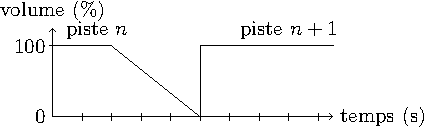
\includegraphics[scale=0.7]{transitions-out.pdf}
  \end{center}
\item s = fade.in(duration=2., s)
  \begin{center}
  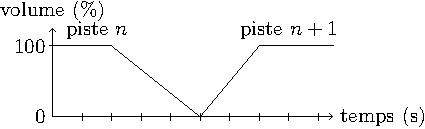
\includegraphics[scale=0.7]{transitions-out-in.pdf}
  \end{center}
\item cross(duration=2., (fun (a,b) -> add([a,b])), s)
  \begin{center}
  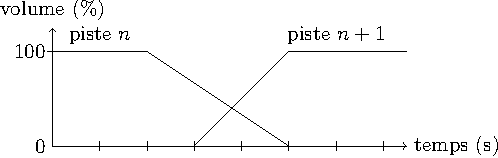
\includegraphics[scale=0.7]{transitions.pdf}
  \end{center}
\end{enumerate}
\end{semiverbatim}
\end{ssl}

\begin{frame}[fragile]
\frametitle{Le langage de script}

%Nous voulons :
\begin{itemize}
\item Un langage fonctionnel (pour les transitions).
\item Des arguments étiquetés et optionnels (pour le confort).
\item Besoin d'analyse statique, intégration de la documentation, simplicité
  d'utilisation.
\end{itemize}
$\Rightarrow$ Création d'un nouveau langage typé et d'un interpréteur.

\bigskip

{\small
\begin{verbatim}
$ liquidsoap -h cross
Generic cross operator, allowing the composition of the
[duration] last seconds of a track with the beginning of the
next track.
Type:
 (?duration:float, ((src, src)->src), src)->src
Parameters:
* duration    :: float (default 5.)
* (unlabeled) :: (src, src)->src    Transition function.
* (unlabeled) :: src
\end{verbatim}}
\end{frame}

\begin{frame}[fragile]
  \frametitle{}
  {\small
\begin{verbatim}
% liquidsoap -h output.icecast.vorbis
Output the source stream as an Ogg Vorbis stream to an Icecast-compatible server in Variable BitRate mode.
Type:
 (?id:string, ?samplerate:int, ?stereo:bool, ?skeleton:bool,
  ?start:bool, ?restart:bool, ?restart_delay:int, ?host:string,
  ?port:int, ?user:string, ?password:string, ?genre:string,
  ?url:string, ?description:string, ?public:bool,
  ?multicast_ip:string, ?sync:bool, ?dumpfile:string,
  ?mount:string, ?name:string, source, ?quality:float)->source
Parameters:
* id :: string (default "")             Force the value of the source ID.
* samplerate :: int (default 44100)
* stereo :: bool (default true)
* skeleton :: bool (default false)      Add an ogg skeleton to the stream. Recommended for theora only.
* start :: bool (default true)          Start output threads on operator initialization.
* restart :: bool (default false)       Restart output after a failure. By default, liquidsoap will stop if the output failed.
* restart_delay :: int (default 3)      Delay, in seconds, before attempting new connection, if restart is enabled.
* host :: string (default "localhost")
* port :: int (default 8000)
* user :: string (default "source")     User for shout source connection. Useful only in special cases, like with per-mountpoint users.
* password :: string (default "hackme")
  ...
* genre :: string (default "Misc")
* url :: string (default "http://savonet.sf.net")
* description :: string (default "OCaml Radio!")
* public :: bool (default true)
* multicast_ip :: string (default "no_multicast")
* sync :: bool (default false)
    Let shout do the synchronization.
* dumpfile :: string (default "")
    Dump stream to file, for debugging purpose. Disabled if empty.
* mount :: string (default "Use [name].ogg")
* name :: string (default "Use [mount]")
* (unlabeled) :: source (default None)
* quality :: float (default 2.)
    Desired quality level, currently from -1. to 10. (low to high).
\end{verbatim}
  }
\end{frame}

\begin{frame}
  \begin{center}
    Comment gérer les étiquettes ?
  \end{center}
\end{frame}

\begin{frame}[fragile]\frametitle{Les étiquettes d'OCaml}
  Les étiquettes d'OCaml sont conçues pour être éliminées à la compilation, ce
  qui entraîne quelques limitations :
% Garrigue parle d'un \emph{sucre syntaxique typé},
{\color{blue}\begin{verbatim}
# let app f = f ~a:1 ~b:2 ;;
val app : (a:int -> b:int -> 'a) -> 'a = <fun>
# app (fun ~b ~a -> a+b) ;;
This function should have type a:int -> b:int -> 'a.
\end{verbatim}}

\onslide<2->

On a besoin d'une multi-application, mais celle-ci ne peut être
$0$-aire en OCaml (d'où les arguments ineffaçables).
{\color{blue}\begin{verbatim}
# let f ?(a=false) () = a ;;
val f : ?a:bool -> unit -> bool = <fun>
# f () ~a:true ;;
- : bool = true
# (f ()) ~a:true ;;
This expression is not a function, it cannot be applied.
\end{verbatim}}
\end{frame}

\begin{frame}
  \begin{itemize}
  \item Dans notre cas, la simplicité passe avant l'efficacité.
  \item On a besoin de formaliser un $\lambda$-calcul avec
    \begin{itemize}
    \item étiquettes,
    \item arguments optionnels,
    \item multi-abstraction et multi-application.
    \end{itemize}
  \end{itemize}
\end{frame}

\begin{ssl}{Termes}
Les termes sont générés par les constructions suivantes:
\begin{eqnarray*}
  M &::=& v \\
  &|& x \\
  &|& \letin{x}{M}{M} \\
  &|& \lambda \{\ldots, l_i:x_i, \ldots, l_j:x_j=M, \ldots\}.M \\
  &|& M\{l_1=M,\ldots,l_n=M\}
\end{eqnarray*}

%Liaisons: $x$ pour le \verb.let. et les $x_i$ pour la multi-abstraction:
%\begin{eqnarray*}
%  x[M/x] &=& M \\
%  y[M/x] &=& y \text{, si $x\neq y$} \\
%  (\letin{y}{N}{P})[M/x] &=& \letin{y}{N[M/x]}{P[M/x]} \\
%  (\lambda \{ \ldots, l_i:y_i,\ldots,l_j:y_j=N_j, \ldots \}. P)[M/x] &=&
%  \lambda \{ \ldots, l_i:y_i,\ldots, l_j:y_j=N_j[M/x], \ldots \}. (P[M/x])
%  \label{rule:subst-abs} \\
%  (N\{ \ldots, l_i=P_i, \ldots\})[M/x] &=& N[M/x]\{\ldots, l_i=P_i[M/x],\ldots \}
%\end{eqnarray*}

Modulo permutation d'étiquettes distinctes :
{\small
\begin{equation*}
  \label{eq:permutation}
  \begin{array}{rcl}
    \lambda \{ \Gamma, l:x, l':x', \Delta \}.M & \equiv &
    \lambda \{ \Gamma, l':x', l:x, \Delta \}.M \\
    \lambda \{ \Gamma, l:x=N, l':x', \Delta \}.M & \equiv &
    \lambda \{ \Gamma, l':x', l:x=N, \Delta \}.M \\
    \lambda \{ \Gamma, l:x=N, l':x'=N', \Delta \}.M & \equiv &
    \lambda \{ \Gamma, l':x'=N', l:x=N, \Delta \}.M
  \end{array}
\end{equation*}
}
(si $l\neq l'$).
\end{ssl}

\begin{ssl}{Réduction}
On a trois règles de réduction:
\[
 \letin{x}{M}{N}
   {\color{red}\;\leadsto\;}
   N[M/x]
\]
L'application peut être \emph{partielle},
  si $\Gamma$ est \emph{ineffaçable}:
\[
 (\lambda\{\vec{l_i:x_i,l_j:x_j=M_j},\Gamma\}.M)\{\vec{l_i=N_i}\}
   {\color{red}\;\leadsto\;}
   \lambda\{\Gamma\}.(M[\vec{N_i/x_i}])
  \]
ou \emph{totale} sinon:
\[
(\lambda\{\vec{l_i:x_i,l_j:x_j=P_j},\vec{l'_k:y_k=M_k}\}.M)\{\vec{l_i=N_i}\}
   {\color{red}\;\leadsto\;}
   M[\vec{N_i/x_i},\vec{M_k/y_k}]
 \]

\begin{block}{Exemple}
\begin{itemize}
  \item $F := \mabs{l_1:x,l_2:y={\color{blue}12},l_3:z={\color{blue}13}}{M}$
  \item $\mapp{F}{l_3={\color{blue}3}} \leadsto \mabs{l_1:x,l_2:y={\color{blue}12}}{M[{\color{blue}3}/z]}$
  \item $\mapp{\mapp{F}{l_3={\color{blue}3}}}{l_1={\color{blue}1}} \leadsto M[{\color{blue}1}/x,{\color{blue}12}/y,{\color{blue}3}/z]$
\end{itemize}
\end{block}
\end{ssl}

\begin{ssl}{Typage}
Les types et schémas de types sont sans surprise:
\begin{equation*}
  t \quad::=\quad \iota
  \quad\mathop{|}\quad \alpha
  \quad\mathop{|}\quad
     \{\ldots, l_i:t_i,\ldots, ?l_j:t_j, \ldots\} \rightarrow t
\end{equation*}
\begin{equation*}
  \sigma\quad ::=\quad t
    \quad\mathop{|}\quad \univ{\alpha}{\sigma} \label{tt:univ}
\end{equation*}

On considère naturellement des règles comme
{\small
\[
  \inferrule{
    \Gamma \vdash M:\{\ldots, l_i:t_i\ldots, ?l_j:t_j,\ldots\}\rightarrow t\\
    \Gamma\vdash N_1:t_1 \\ \cdots \\ \Gamma\vdash N_n:t_n}
  {\Gamma \vdash M \{ \ldots, l_i=N_i, \ldots, l_j=N_j, \ldots \} : t }{
   \regle{App}}
\]
}
ou encore
{\small
\[
  \inferrule
  {
    \Gamma, \ldots, x_i:t_i, \ldots, x_j:t_j, \ldots \vdash M : t
    \\ \cdots \\
    \Gamma\vdash M_j:t_j
    \\ \cdots
  }
  {
    \Gamma\vdash\lambda\{ \ldots, l_i:x_i,\ldots, l_j:x_j=M_j, \ldots \}.M
    : \{ \ldots, l_i:t_i,\ldots, ?l_j:t_j,\ldots \} \rightarrow t}
  {\regle{Abs}}
\]
}
\end{ssl}

\begin{ssl}{Sous-typage et application partielle}

  La réduction permet l'application partielle. Le système de type, pas encore :
  une fonction de type $\tmabs{l_1:t_1,l_2:t_2}{t}$ doit pouvoir être considérée
  comme une fonction de type $\tmabs{l_1:t_1}{\tmabs{l_2:t_2}{t}}$.

  \[
  \inferrule{\mbox{$\Delta$ ineffaçable}}{
    \{ \Gamma, \Delta \}\rightarrow t {\color{red}\leq}
    \{\Gamma\}\rightarrow\{\Delta\}\rightarrow t
  }
  \qquad
  \inferrule{\mbox{$\Delta$ effaçable}}{
    \{ \Gamma, \Delta \}\rightarrow t {\color{red}\leq} \{\Gamma\}\rightarrow t
  }
  \]

  \onslide<2->
  \bigskip
  Quelques équations invalides :
  \begin{itemize}
  \item $
    \tmabs{l_1:t_1}{\tmabs{l_2:t_2}{t}}
    {\color{red}\not\leq}
    \tmabs{l_1:t_1,l_2:t_2}{t}
    $
  \item $\tmabs{\Gamma,?l:t,\Delta}{t'} {\color{red}\not\leq}
    \tmabs{\Gamma,l:t,\Delta}{t'}$
  \end{itemize}
\end{ssl}

\begin{frame}
  \frametitle{$\tmabs{\Gamma,?l:t,\Delta}{t'} {\color{red}\not\leq}
    \tmabs{\Gamma,l:t,\Delta}{t'}$}


  Par exemple, considérons le terme $f$ suivant
  \[
  \mabs{l:x=5}{x}\quad:\quad\tmabs{?l:int}{int}
  \]
  On ne peut pas calculer
  \[
  \mapp{\mapp{f}{}}{l=6}
  \]
  donc on n'a pas
  \[
  \mabs{l:x=5}{x}\quad:\quad\tmabs{l:int}{int}
  \]
\end{frame}

\begin{frame}
  \frametitle{Quelques propriétés du calcul}
  \begin{itemize}
  \item Le calcul pur est confluent.
  \item Subject reduction.
  \item Les termes typables sont terminants.
  \end{itemize}
\end{frame}

\begin{ssl}{Inférence}
  \begin{itemize}
  \item Une variante de l'algorithme W de Damas-Milner.
  \item<2-> Il n'y a pas de type principal : $\mabs{l:g}{\mapp{g}{l'=42}}$ admet
    \[
    \univ\alpha{\tmabs{l:\tmabs{l':int}\alpha}\alpha}
    \]
    et
    \[
    \univ\alpha{\tmabs{l:\tmabs{?l':int}\alpha}\alpha}
    \]
    comme types.
    \item<3-> Cependant, on peut plonger les termes
      \[
      f
      \quad:\quad
      \tmabs{?l:int}\alpha
      \]
      dans
      \[
      \mabs{l:x}{\mapp{f}{l=x}}
      \quad:\quad
      \tmabs{l:int}\alpha
      \]
  \end{itemize}
\end{ssl}

\begin{frame}
  \frametitle{Remarque : variante avec types principaux}

  Décomposer la multi-application en
  \begin{itemize}
  \item une multi-application partielle
    \[
    \mapp{(\mabs{\vec{l_i:x_i,l_j:x_j=M_j},\Gamma}{M})}{\vec{l_i=N_i}}
    \leadsto
    \lambda\{\Gamma\}.(M[\vec{N_i/x_i}])
    \]
  \item une destruction des multi-abstractions effaçables
    \[
    (\mabs{\vec{l_i:x_i=M_i}}{M})\bullet
    \leadsto
    M[\vec{M_i/x_i}]
    \]
  \end{itemize}
\end{frame}

\partie{Implémentation}

\begin{frame}
  \frametitle{Le code}

  \begin{itemize}
  \item Implémenté en OCaml (et en C)
  \item Savonet (OCaml : 60 kLOC, C : 15 kLOC)\\
    Liquidsoap (OCaml : 35 kLOC, C : 1.8 kLOC)
  \item Plus de 30 librairies :
    \begin{itemize}
    \item formats audio (mad+lame, ogg/vorbis, aac, speex, \ldots + tags)
    \item carte son (alsa, ao, pulseaudio, portaudio, \ldots)
    \item effets audio (ladspa, samplerate, \ldots)
    \item transmission audio (jack, shout)
    \item autres (lastfm, irc)
    \end{itemize}
  \end{itemize}
\end{frame}

\begin{frame}
  \frametitle{Les flux}

  \begin{itemize}
  \item Pas d'accès direct depuis le langage.
  \item Découpés en \textbf{buffers}\\
    (perfs vs realtime)
  \item de type \texttt{float array}\\
    (endianness, précis, non boxé, tout en OCaml)
  \item Il faut gérer les buffers partiels
  \item On partage et réutilise les buffers pour éviter les copies\\
    (mais problèmes de temporalités)
  \end{itemize}
\end{frame}

\begin{frame}
  \frametitle{Interaction avec l'extérieur}
  \begin{itemize}
  \item Playlists dynamiques
  \item Telnet (ou socket)
    \begin{itemize}
    \item queues de requêtes
    \item variables
    \end{itemize}
  \item Métadonnées (ex : replaygain, transitions)
  \end{itemize}

  \bigskip

  Tout est envisageable : sites web, bots IRC, etc.
\end{frame}

\begin{frame}[fragile]
  \frametitle{Gestion des ``fichiers''}

  Il faut en particulier
  \begin{itemize}
  \item télécharger les fichiers distants en avance,
  \item gérer les flux web,
  \item protocoles extensibles avec plusieurs résolutions\\
    (\verb+say://+, \verb+replaygain://+, \verb+strider://+, \ldots)
  \end{itemize}
\end{frame}

\begin{frame}
  \frametitle{Le présent}

  La version SVN de Liquidsoap a le support de la \textbf{vidéo}.
  \begin{itemize}
  \item Bon point : ça rentre très facilement dans notre cadre
  \item De nouveaux problèmes :
    \begin{itemize}
    \item la synchronisation entre les pistes du flux
    \item il faut \emph{vraiment} être efficace :
      \[
      640 \times 480 \times 4 \times 24 \quad\approx\quad 30\text{ Mo/s}
      \]
      (en particulier encodage et YUV$\to$RGB)\\
      $\Rightarrow$ codé en C, \texttt{gcc} avec optimisations
    \end{itemize}
  \end{itemize}

\end{frame}

\begin{frame}
  \frametitle{Le futur}

  \begin{itemize}
  \item Gérer les flux hétérogènes de façon typée :
    \begin{itemize}
    \item des flux que audio ou que vidéo (canaux, résolution, \ldots)
    \item des flux compressés
    \item etc.
    \end{itemize}
  \item Gérer finement les partages (avec des boîtes dans le typage ?)
  \end{itemize}
\end{frame}


\begin{ssl}{Conclusion}
\begin{itemize}
\item Une variante originale du $\lambda$-calcul.
\item<2-> Beaucoup de composants réutilisables.
\item<3-> Un langage
  \begin{itemize}
  \item purement fonctionnel
  \item statiquement typé
  \item programmé en OCaml
  \end{itemize}
  qui commence à être utilisé (par des non-programmeurs).
\item<4-> Démo par David\ldots
\end{itemize}
\end{ssl}

\end{document}
